\documentclass[../report.tex]{subfiles}
\begin{document}
	
\subsection{Seismic Waves} \label{sec:seismicwaves}
	Seismic waves take on two main forms, body waves and surface waves.  Body waves are those that travel through the interior of the earth and are the fastest travelling.  The body waves are comprised of \textbf{P} (primary) waves which are compressional waves, travel fastest and thus arrive first.  \textbf{S} (secondary) waves are shear waves and travel more slowly, thus arrive later.  The separation between the phases is related to the distance of the earthquake and the local velocity structure. The surface waves travel only along the earth's crust and, as they are confined to shallow depths where seismic velocities are slow, will normally arrive much later than the body waves.
	
	A seismic station records movement over three axis: vertical (\textbf{z}) alongside horizontal in terms of north-south (\textbf{n}) and east-west (\textbf{e}).  Due to seismic velocities generally increasing with depth, P waves arrive at a seismic station close to the vertical axis.  As a result, P waves can be measured as a simple metric of displacement along the Z axis.  S waves follow similar ray paths, but have their particle motion perpendicular to the direction of propagation.  As a result, they manifest on a seismogram as movement on both the \textbf{n} and \textbf{e} axis. The geometry of the fault tends to have a bearing on the orientation of the displacement so the two horizontal axis of movement cannot be easily combined in to a single metric for time series analysis.
	
	There are three main factors that will affect the final signal recorded at a station.  The first is the fault geometry itself, this means that depending on the angle of the fault, The phase and amplitude of the originating signal depend on the angle of the station relative to the fault as shown in \cref{fig:faultangle}.  The effects on amplitude should be eliminated by normalisation but the phase may require special care in pattern matching.
	
\begin{figure}[H]
	\centering
	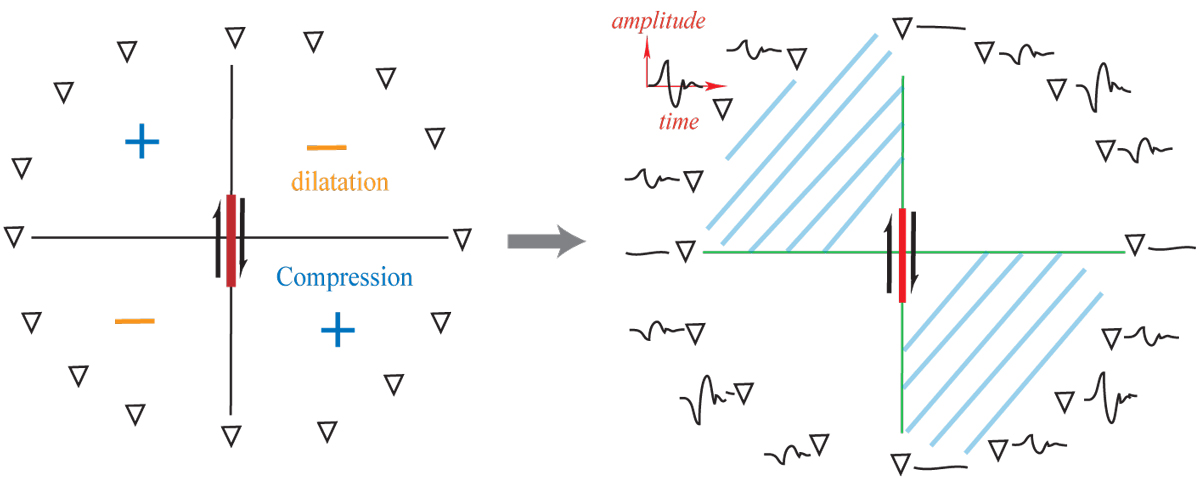
\includegraphics[width=1\linewidth]{img/fault_angle}
	\caption{Effect of fault geometry on amplitude and phase \citep{faultangle}}
	\label{fig:faultangle}
\end{figure}

	The second factor is the path effect.  This is what happens to the signal as it passes though various substrates and geological boundaries.  It produces a not easily predictable effect on the velocity, amplitudes and frequencies of a wave as it passes through them.  In addition, the boundaries can cause reflection and refraction of the signals further distorting the recorded signal at a station.
	
	The final factor is the frequency response and characteristics of the station itself.  In the main dataset from the Nabro Volcano \citep{eritrea1}, this can be largely ignored as the stations are all of the same make and model however should be considered when looking at datasets involving many differing stations.

\end{document}